\section{半导体中的缺陷}
在本节,我们主要半导体中研究点缺陷和线缺陷,尤其是缺陷造成的缺陷能级。

\subsection{点缺陷}
在固体物理中曾提到过,\uwave{点缺陷}(Point Defect)包含两种
\begin{itemize}
    \item \uwave{肖特基缺陷}(Schottky Defect),在晶体中仅产生空位,如\xref{fig:肖特基缺陷}所示。
    \item \uwave{弗伦克尔缺陷}(Frenkel defect),在晶体中成对产生空位和填隙原子,如\xref{fig:弗伦克尔缺陷}所示。
\end{itemize}

\begin{Figure}[点缺陷]
    \begin{FigureSub}[肖特基缺陷]
        \includegraphics{build/Chapter02B_01.fig.pdf}
    \end{FigureSub}
    \hspace{1.5cm}
    \begin{FigureSub}[弗伦克尔缺陷]
        \includegraphics{build/Chapter02B_02.fig.pdf}
    \end{FigureSub}
\end{Figure}

肖特基缺陷和弗伦克尔缺陷总是同时存在的,由于原子需要由较大的能量才能挤入同种原子构成晶体的间隙位置,所以实际上,空位比间隙原子要多得多,空位是更常见的点缺陷。

那么,空位和间隙原子是如何产生能级的呢?在硅和锗中
\begin{itemize}
    \item 空位会表现为受主性质,因为,注意到,空位的存在使得其邻近的四个原子各有一个不成对的电子,是不饱和的共价键,这些键可以接受电子,从而表现出受主性质。
    \item 间隙原子会表现为施主性质,因为间隙原子未成键,有四个价电子可以失去。
\end{itemize}
这样,空位和间隙原子的效果,就可以并入到我们已经很熟悉的受主和施主的框架内了。

\subsection{线缺陷}
在这里,我们要讨论的\uwave{线缺陷}(Line Defect)主要是指\uwave{位错}(Dislocation)\cite{W9}。

如\xref{fig:位错的分类}所示\cite{W7},位错可以分为两类
\begin{itemize}
    \item \uwave{刃形位错}(Edge Dislocation)是\xref{fig:位错的分类}的左图所示的情形。形象的说,刃形位错就是在原先排列规整的晶格中,用刀刃切开一个口子,强行塞入一个半晶面,而该半晶面会在晶体内部突然终止于某一条线处(取决于切的有多深),这条线就是所谓的位错线。
    \item \uwave{螺形位错}(Screw Dislocation)是\xref{fig:位错的分类}的右图所示的情形。形象的说,螺形位错就是将晶体用剪刀剪开,将一侧向上拉,将一侧向下拉,使得剪刀剪开的切面两侧发生滑移。
\end{itemize}
位错可以通过两个矢量研究,其中一个是前面已经提到的位错线$\vb*{L}$,还有一个称为\uwave{伯格斯矢量}(Burgers Vector),记为$\vb*{b}$,伯格斯矢量是指,由于位错的引入,在垂直位错线的晶面上的回路将会发生扭曲,在原有的回路的中间附加了一个矢量,这个矢量就是伯格斯矢量,从这种矢量的观点上看,刃形位错即$\vb*{L},\vb*{b}$垂直的位错,螺形位错即$\vb*{L},\vb*{b}$平行的位错,而若位错线和伯格斯矢量既不平行也不垂直,那就可以视为刃形位错和螺形位错的组合,称为\uwave{混合位错}。

\begin{Figure}[位错的分类]
    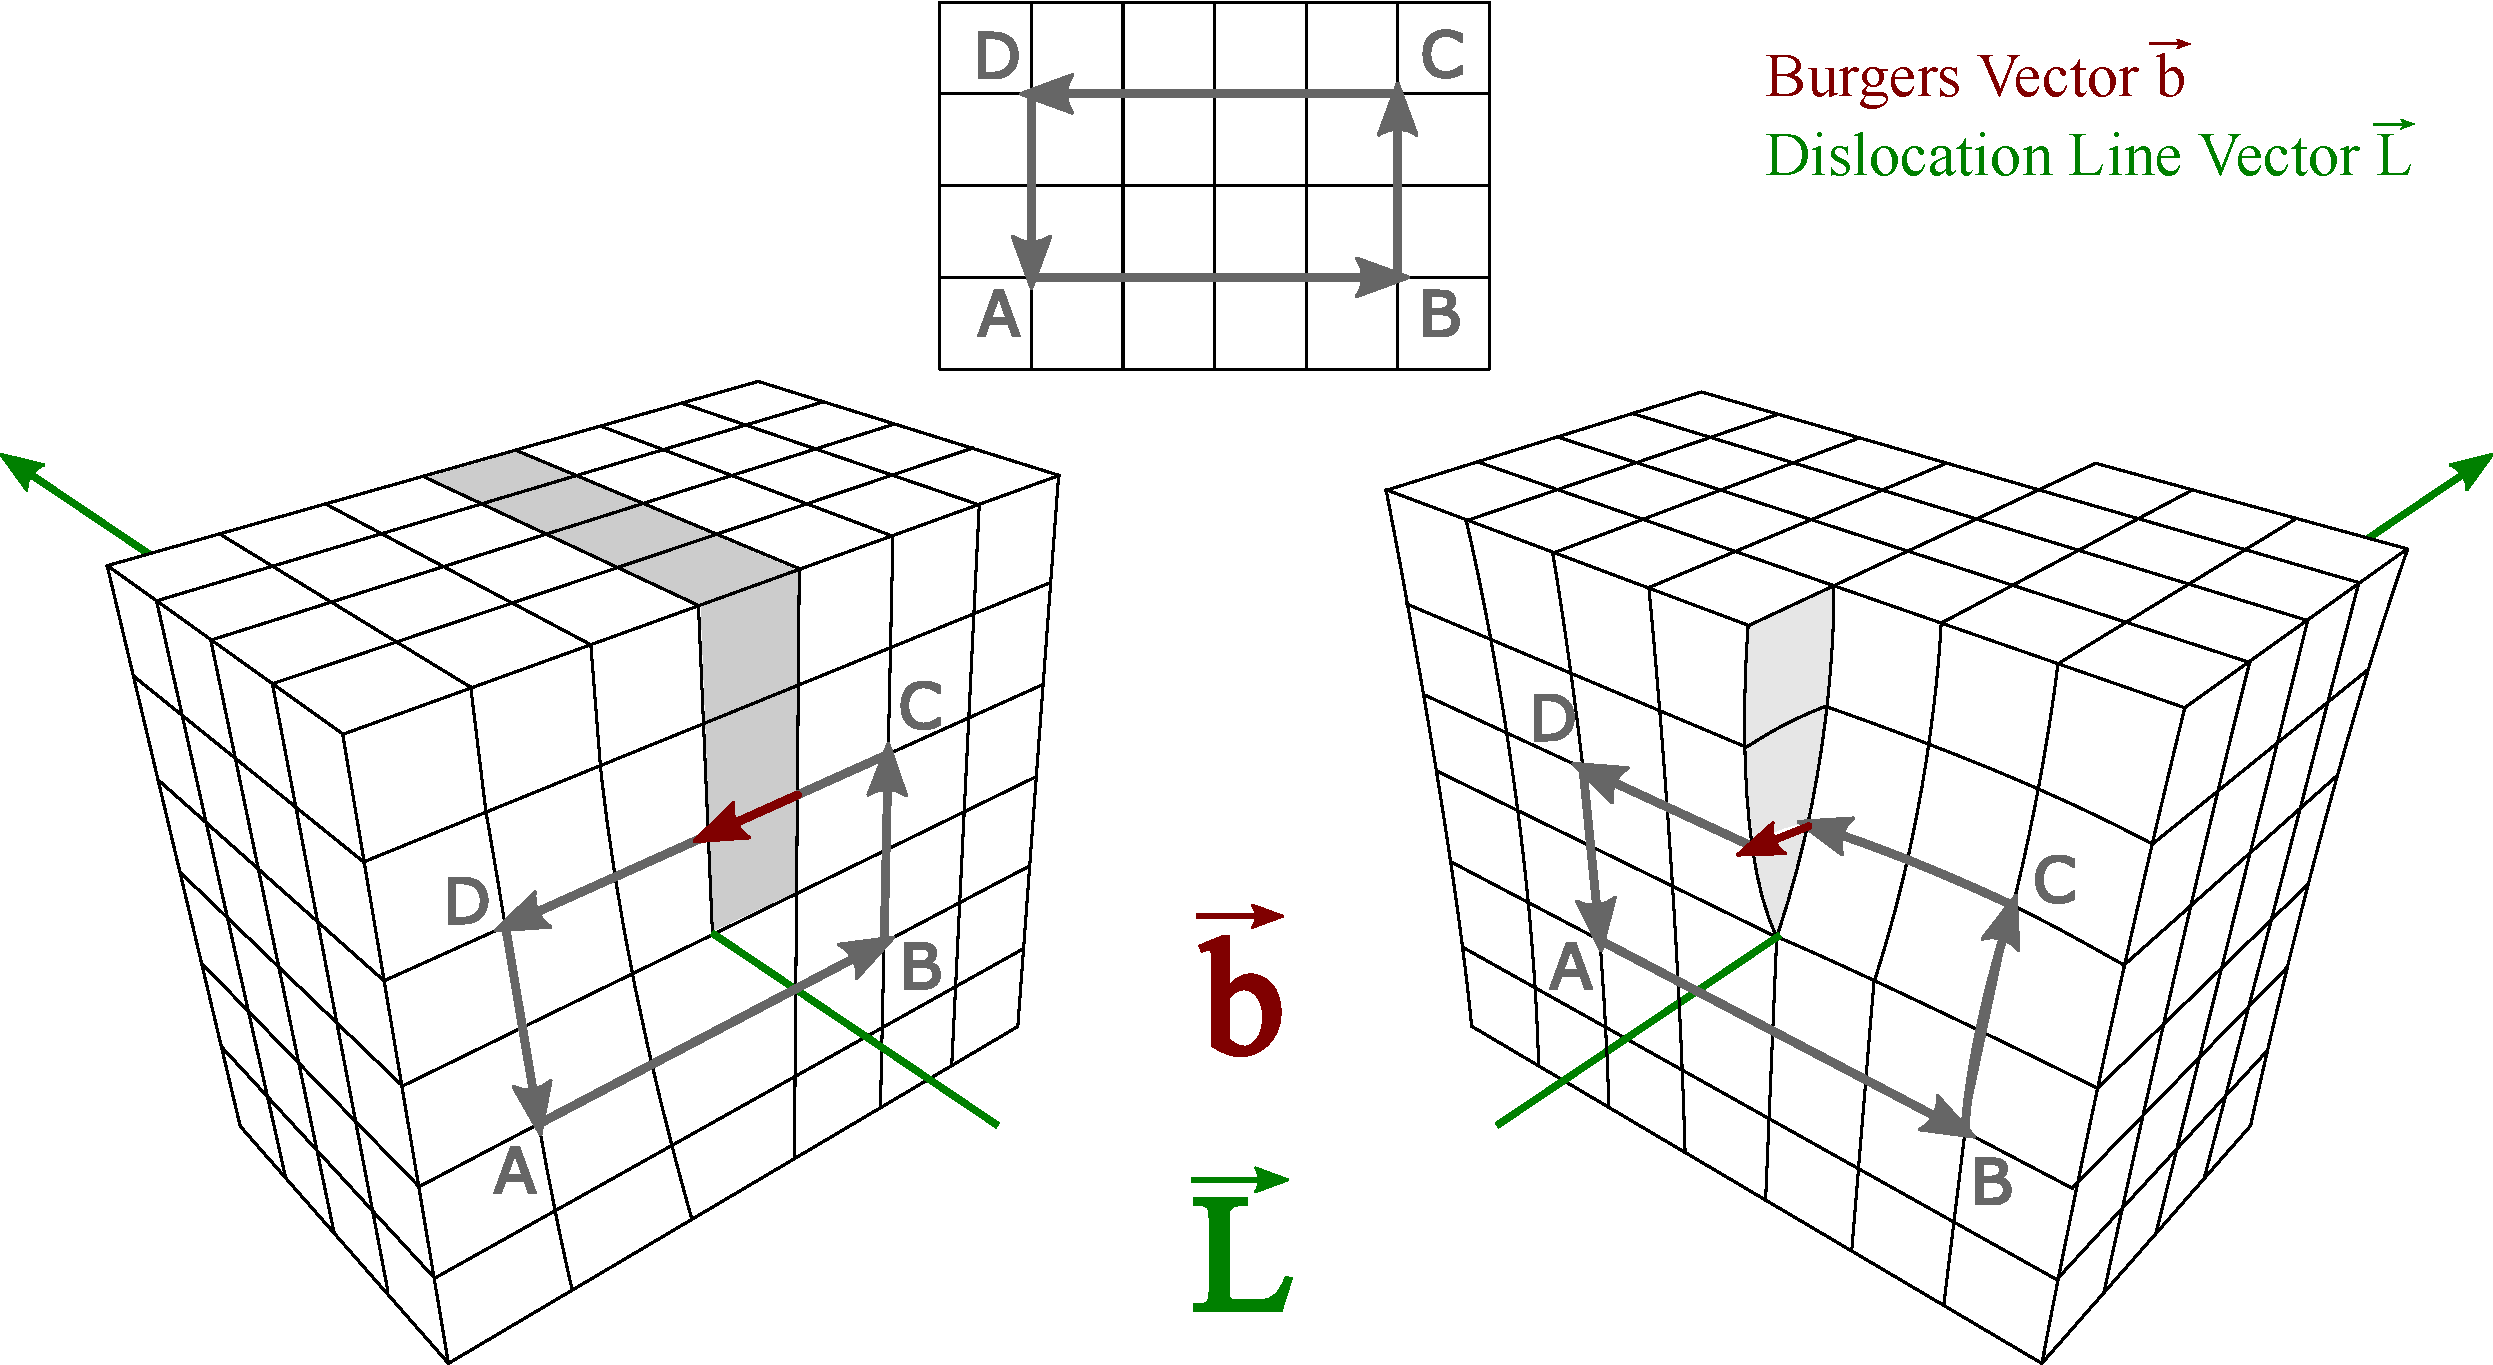
\includegraphics[width=10cm]{image/Burgers_Vector_and_dislocations.pdf}
\end{Figure}

位错是如何影响半导体的性质的呢,如\xref{fig:位错的影响}所示\cite{W8},这是垂直位错线的一个晶体截面,以橙色文字和$E$标注的就是位错线落在该截面上的原子,称为位错核心。位错核心$E$仅与三个原子成键,还有一个电子,它既可以接受电子作为受主,它也可以失去电子作为施主,而这种位错核心的原子存在于整条位错线上,因此,我们说,位错意味着一串施主原子或受主原子。
\begin{Figure}[位错的影响]
    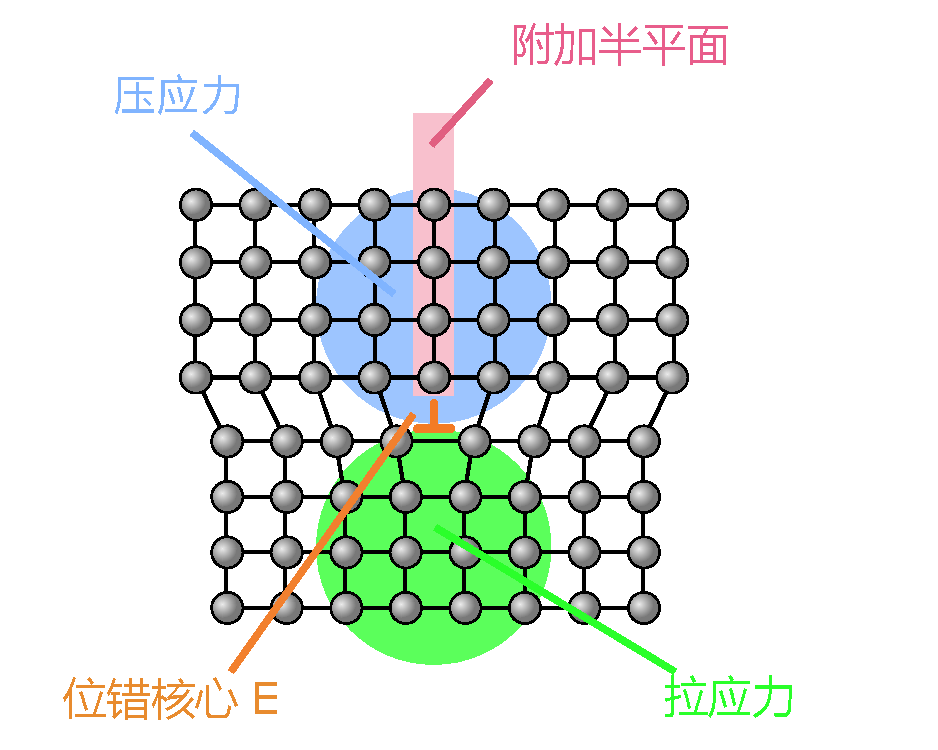
\includegraphics[width=6.5cm]{image/Versetzung_im_2D-Kristall.pdf}
\end{Figure}

理论指出,发生位错时,导带底$E_\text{c}$和价带顶$E_\text{v}$的改变量为\setpeq{线缺陷}
\begin{Align}[8pt]
    \delt{E_\text{c}}&=E_\text{c}-E_\text{c0}=\varepsilon_\text{c}\frac{\delt{V}}{V_0}\xlabelpeq{1}\\
    \delt{E_\text{v}}&=E_\text{v}-E_\text{v0}=\varepsilon_\text{v}\frac{\delt{V}}{V_0}\xlabelpeq{2}
\end{Align}

这里$\varepsilon_\text{c},\varepsilon_\text{v}$是单位体积形变引起的$E_\text{c},E_\text{v}$的变化,是有关材料的常数,称为\uwave{形变势常数}。

因此禁带宽度变化可以表示为
\begin{Equation}&[3]
    \delt{E_\text{g}}=(\varepsilon_\text{c}-\varepsilon_\text{v})\frac{\delt{V}}{V_0}
\end{Equation}
换言之,禁带宽度的变化量,与单位体积的形变成正比,事实上
\begin{itemize}
    \item 在位错线以上的伸张区,形变为正(压应力,向外挤压晶格),禁带宽度减小。
    \item 在位错线以下的压缩区,形变为负(拉应力,向内拉紧晶格),禁带宽度增大。
\end{itemize}

按照这个结论,应有$\varepsilon_\text{c}-\varepsilon_\text{v}<0$成立?这一部分的逻辑关系有待进一步梳理。
